\documentclass[aip,apl]{revtex4-1}
\usepackage{fontspec}
\usepackage{amsmath,bm,amsfonts,amssymb}
\usepackage{graphicx}
\usepackage{tikz}
\usepackage[colorlinks=true,
			linkcolor=blue,
			citecolor=blue,
			urlcolor=blue]
			{hyperref}
\usepackage{subcaption}
\usepackage{placeins}
\usepackage{cleveref}
\usepackage{minted}
\usepackage{lmodern}

\begin{document}
	\title{Study of plasma recombination in Debye sheaths}
	\author{Daniel Celis Garza}
	\email{daniel.celisgarza@materials.ox.ac.uk}
	\affiliation{Department of Materials, University of Oxford}
	\begin{abstract}
		\begin{itemize}
			\item Summarises main results
			\item Brief and to the point
			\item Guidline length 1-2 paragraph(s)
			\item 10\%
		\end{itemize}
	\end{abstract}
	\maketitle
	
	\section{Introduction}
	\begin{itemize}
		\item Brief overview of literature
		\item Motivates current study
		\item Guidline length $\dfrac{1}{2}$ page
		\item 10\%
	\end{itemize}
	
	\section{Results}
	\begin{figure}
		\centering
		\begin{subfigure}[b]{\textwidth}
			\centering
			\foreach \x in {0,1}
			{
				\includegraphics[width=0.3\linewidth]{\x_-1l.eps}
				~
			}
			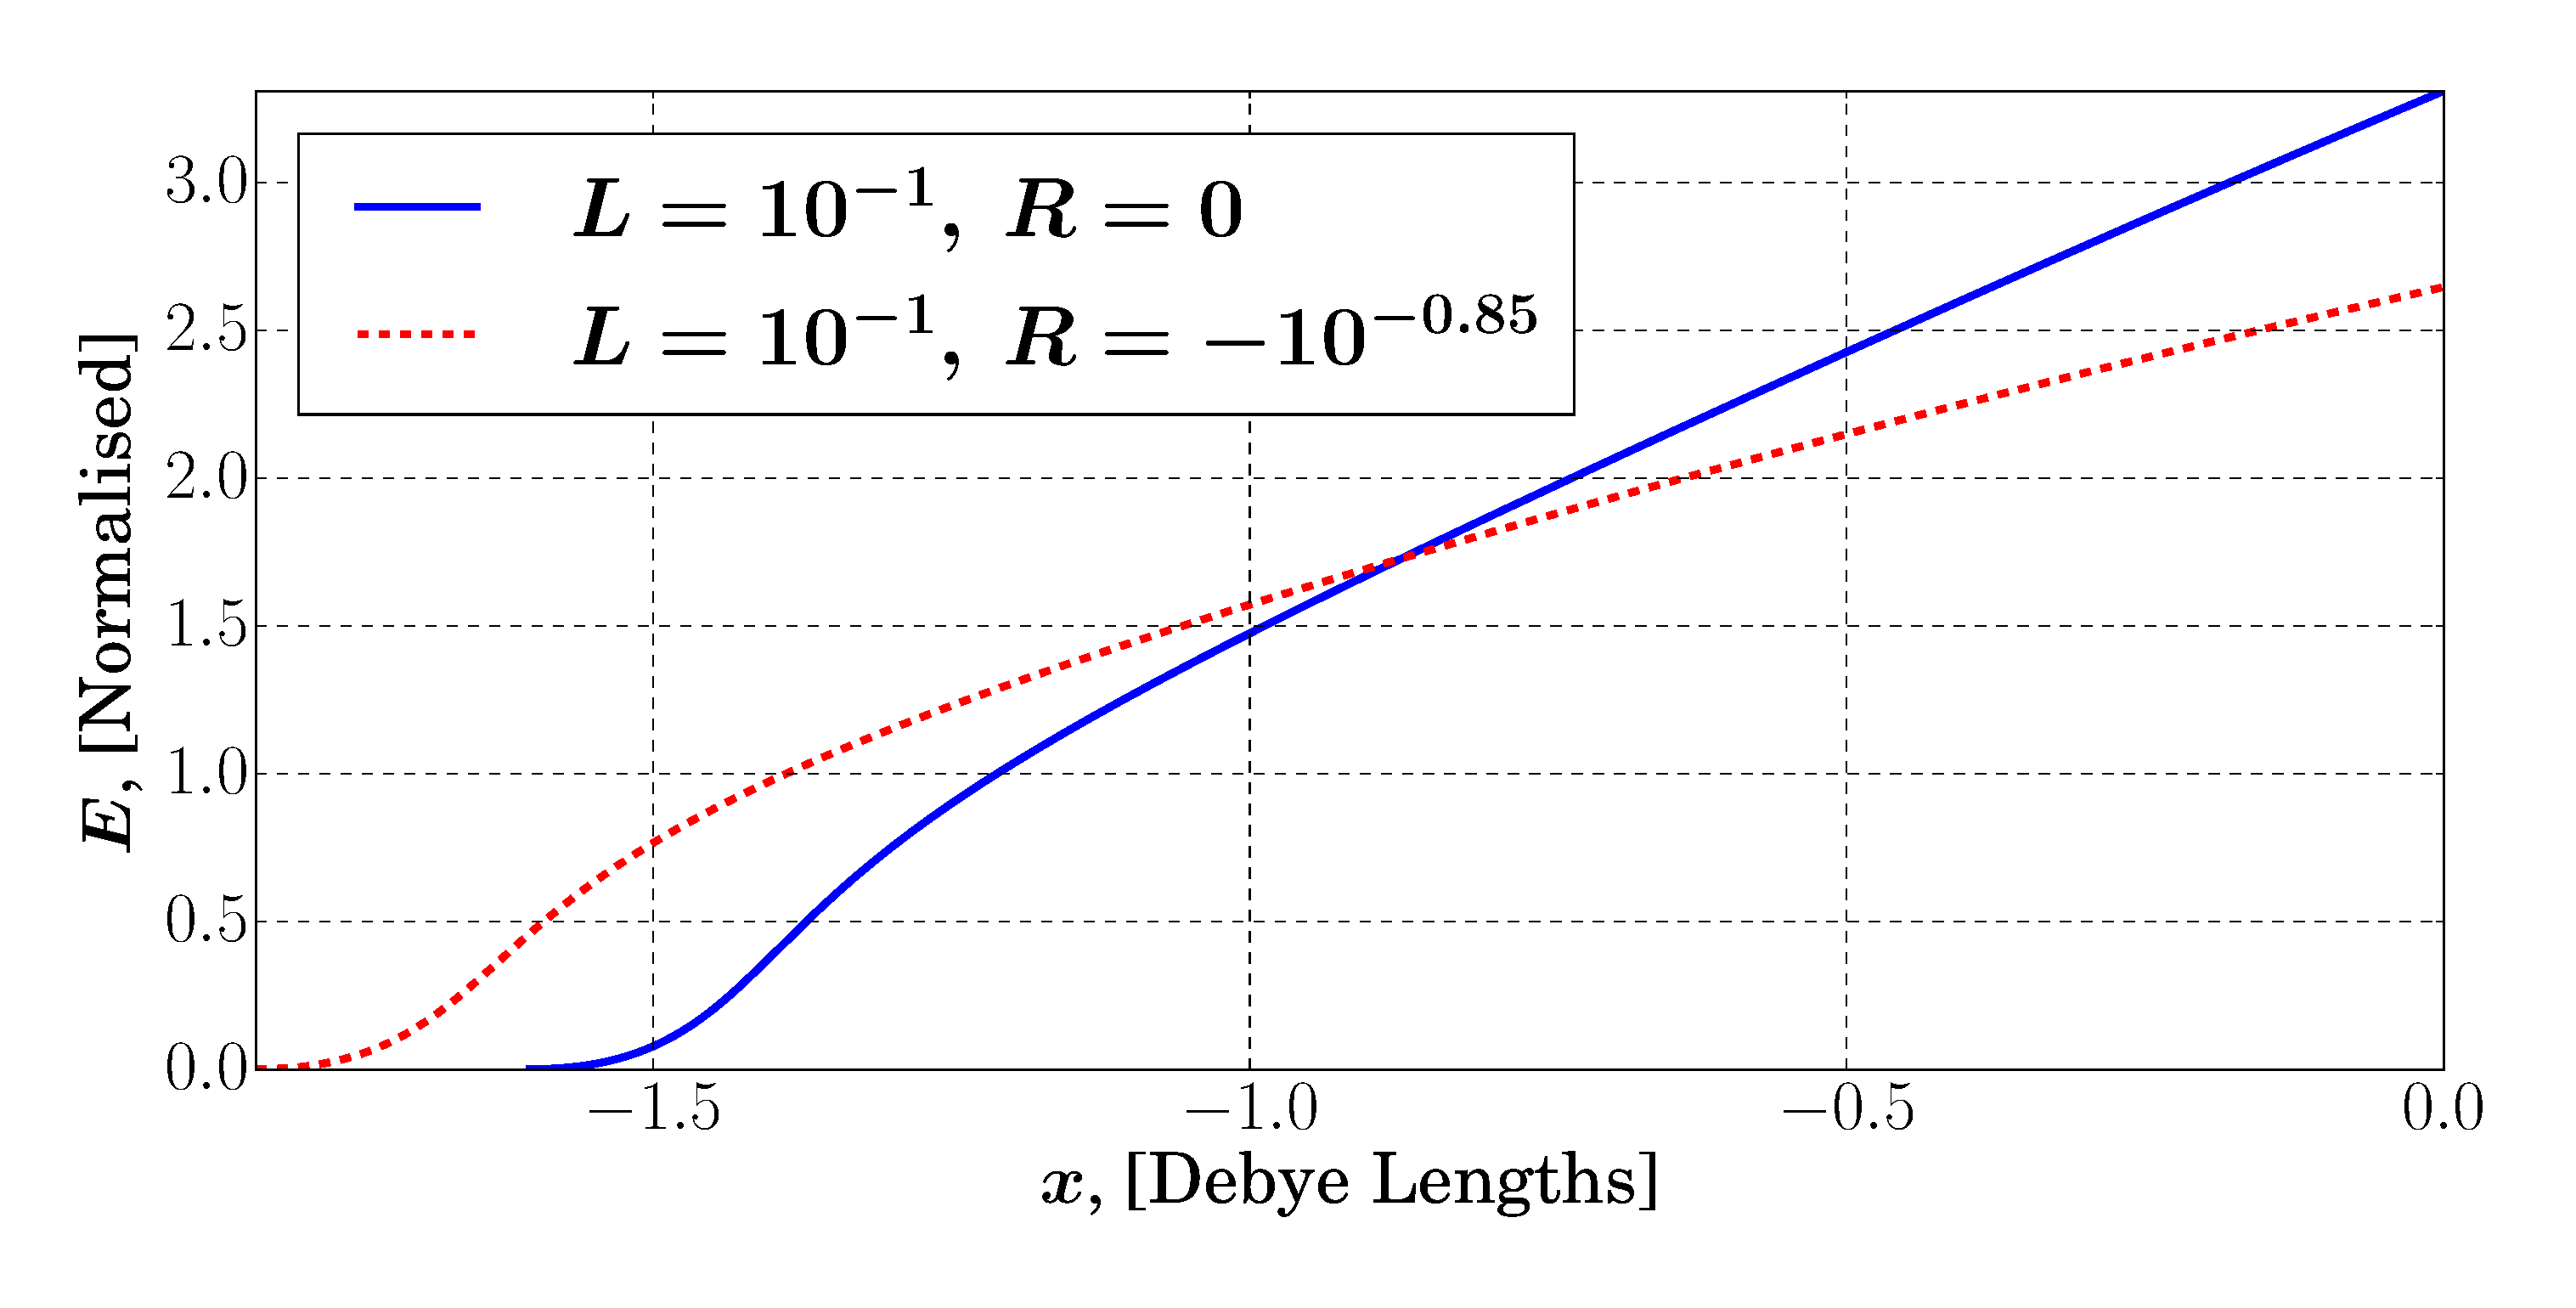
\includegraphics[width=0.3\linewidth]{2_-1l.eps}
			
			\foreach \x in {3,4}
			{
				\includegraphics[width=0.3\linewidth]{\x_-1l.eps}
				~
			}
			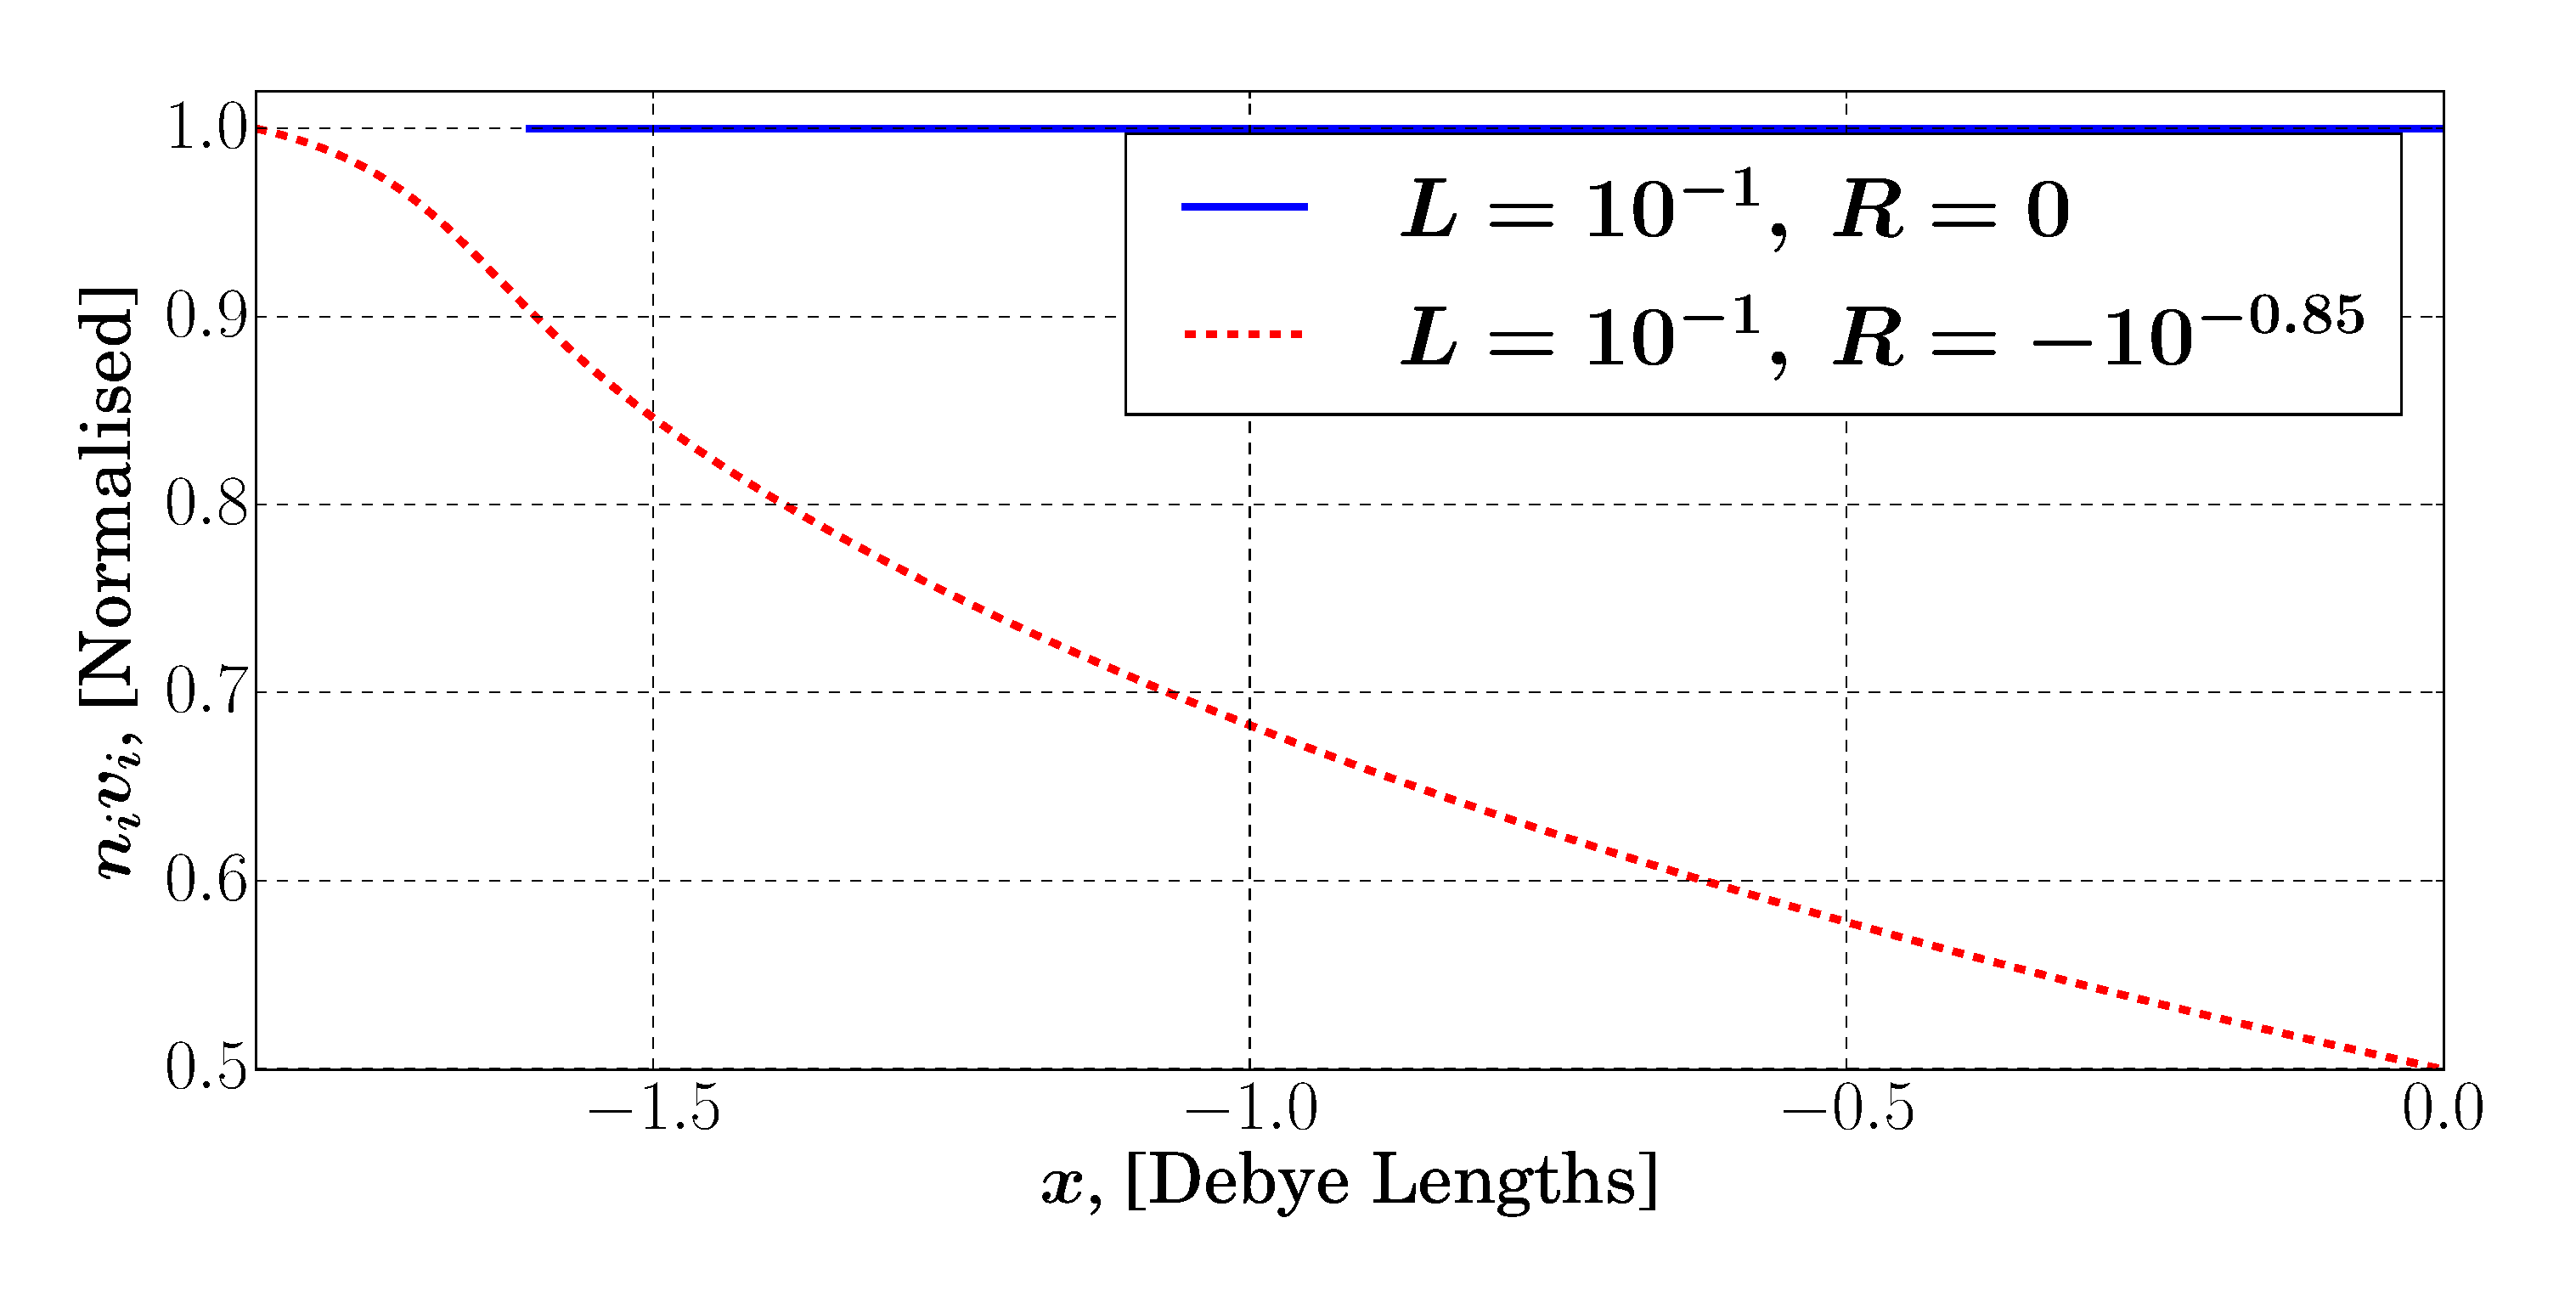
\includegraphics[width=0.3\linewidth]{6_-1l.eps}
			\caption{$ L = 10^{-1} $.}
		\end{subfigure}
		
		\begin{subfigure}[b]{\textwidth}
			\foreach \x in {0,1}
			{
				\includegraphics[width=0.3\linewidth]{\x_1l.eps}
				~
			}
			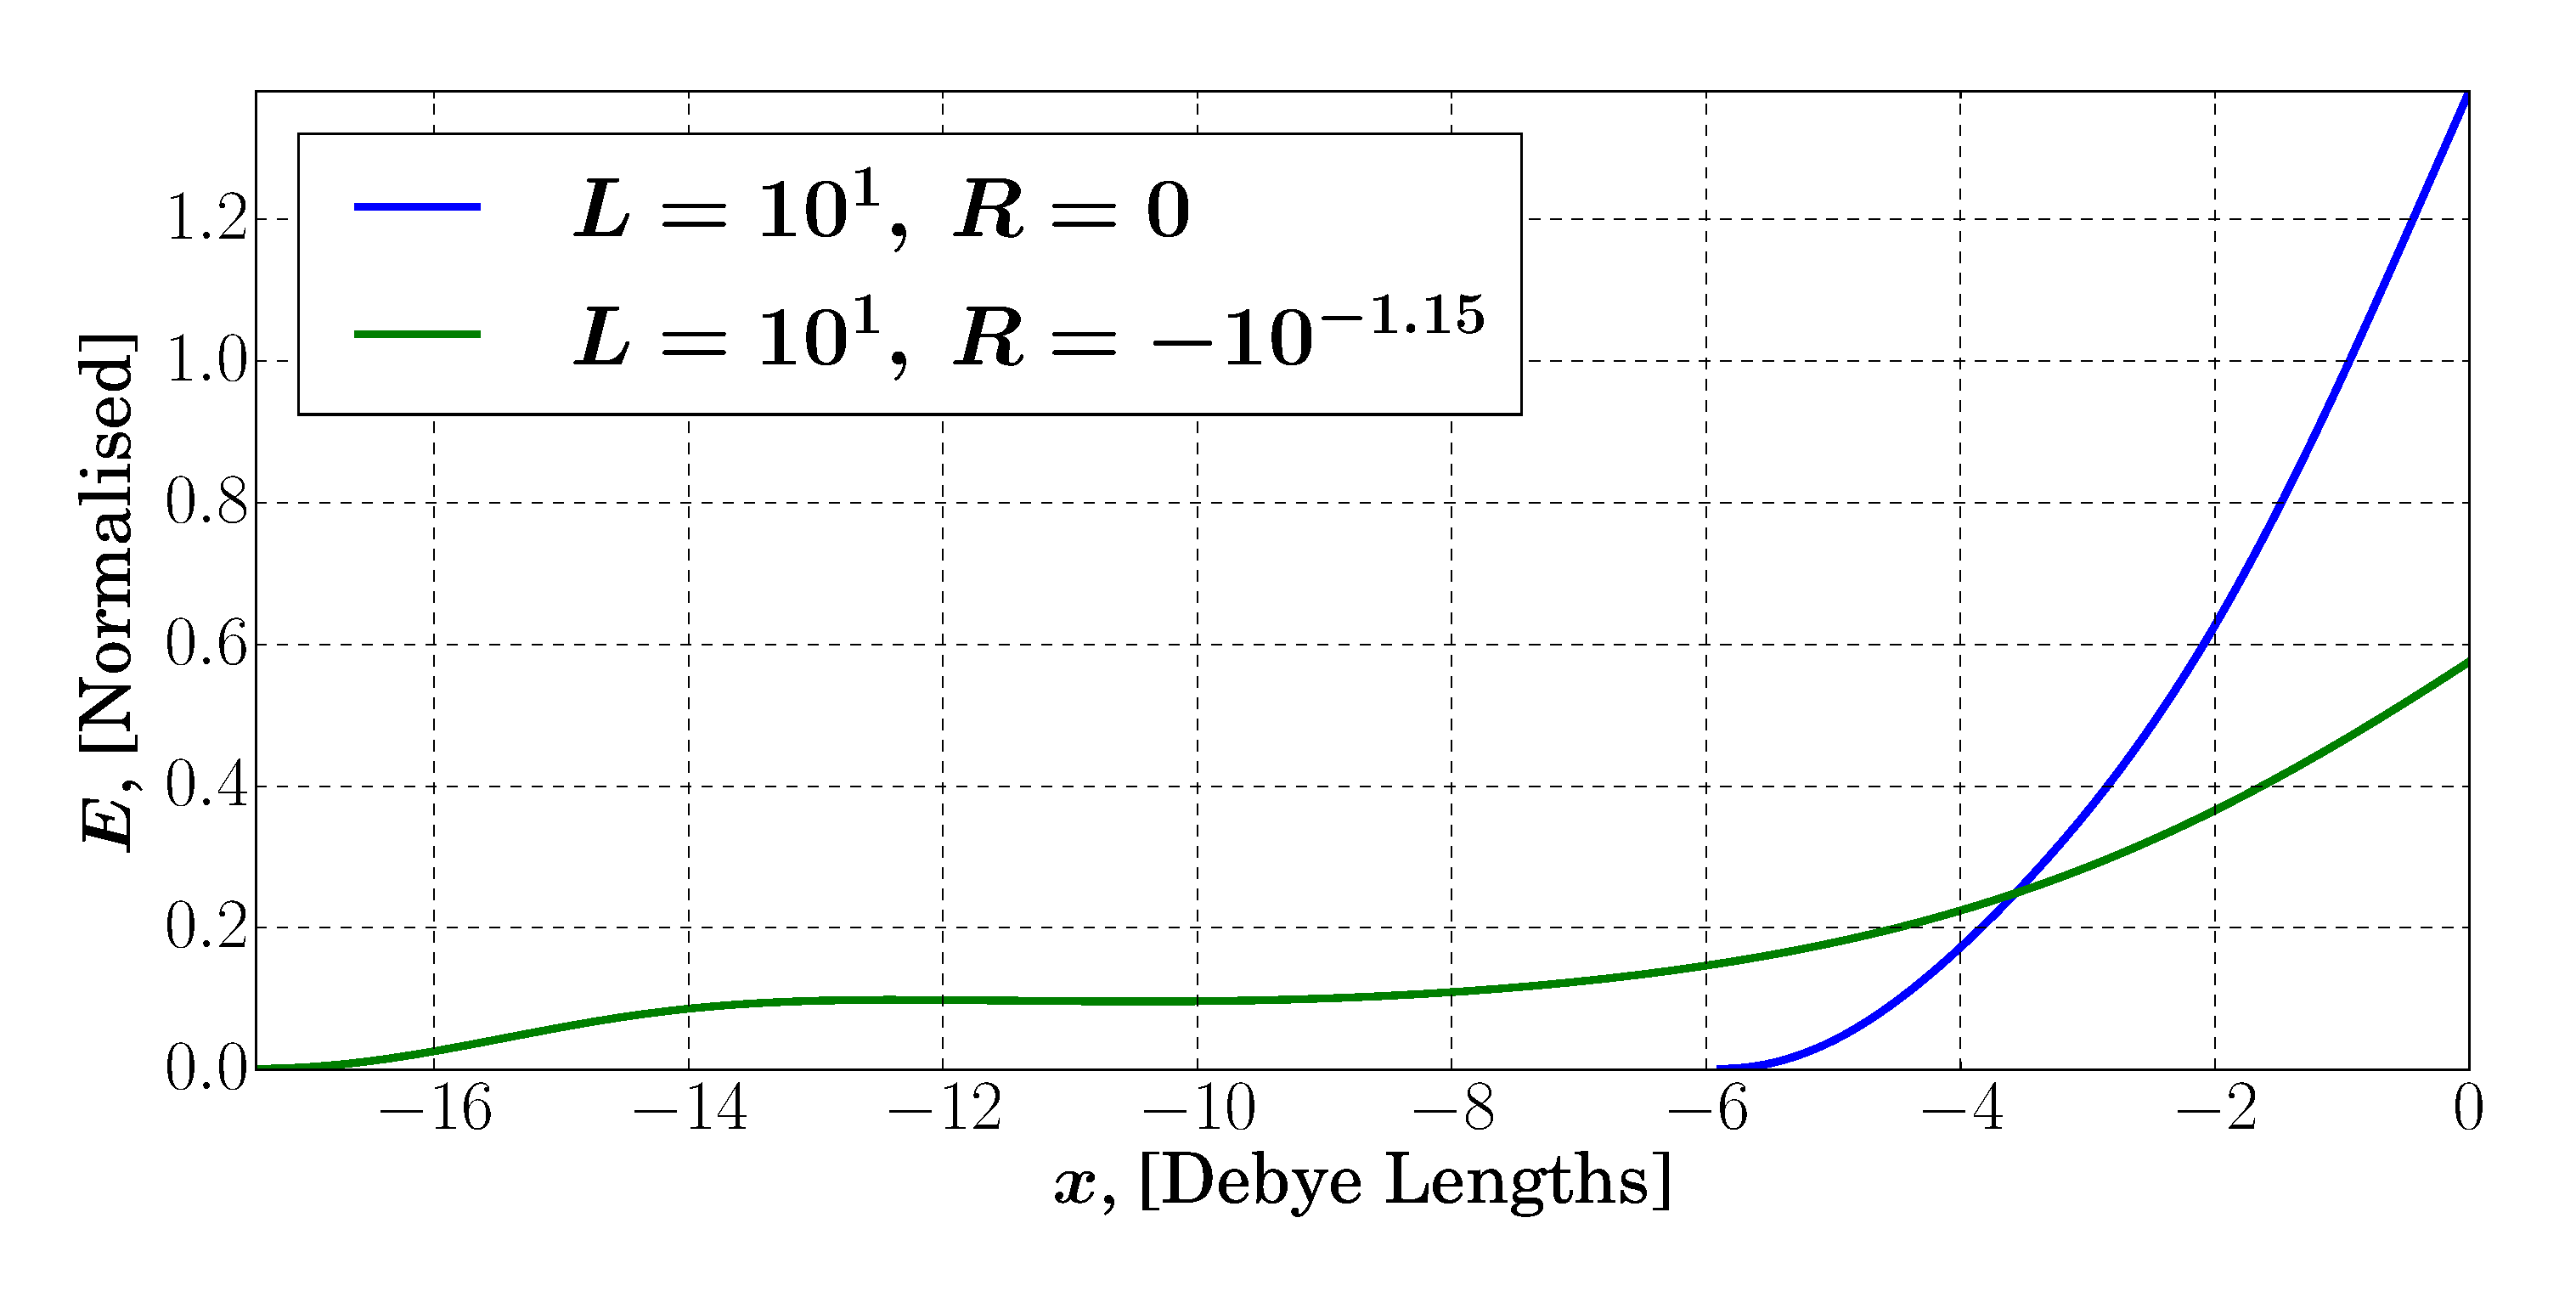
\includegraphics[width=0.3\linewidth]{2_1l.eps}
			
			\foreach \x in {3,4}
			{
				\includegraphics[width=0.3\linewidth]{\x_1l.eps}
				~
			}
			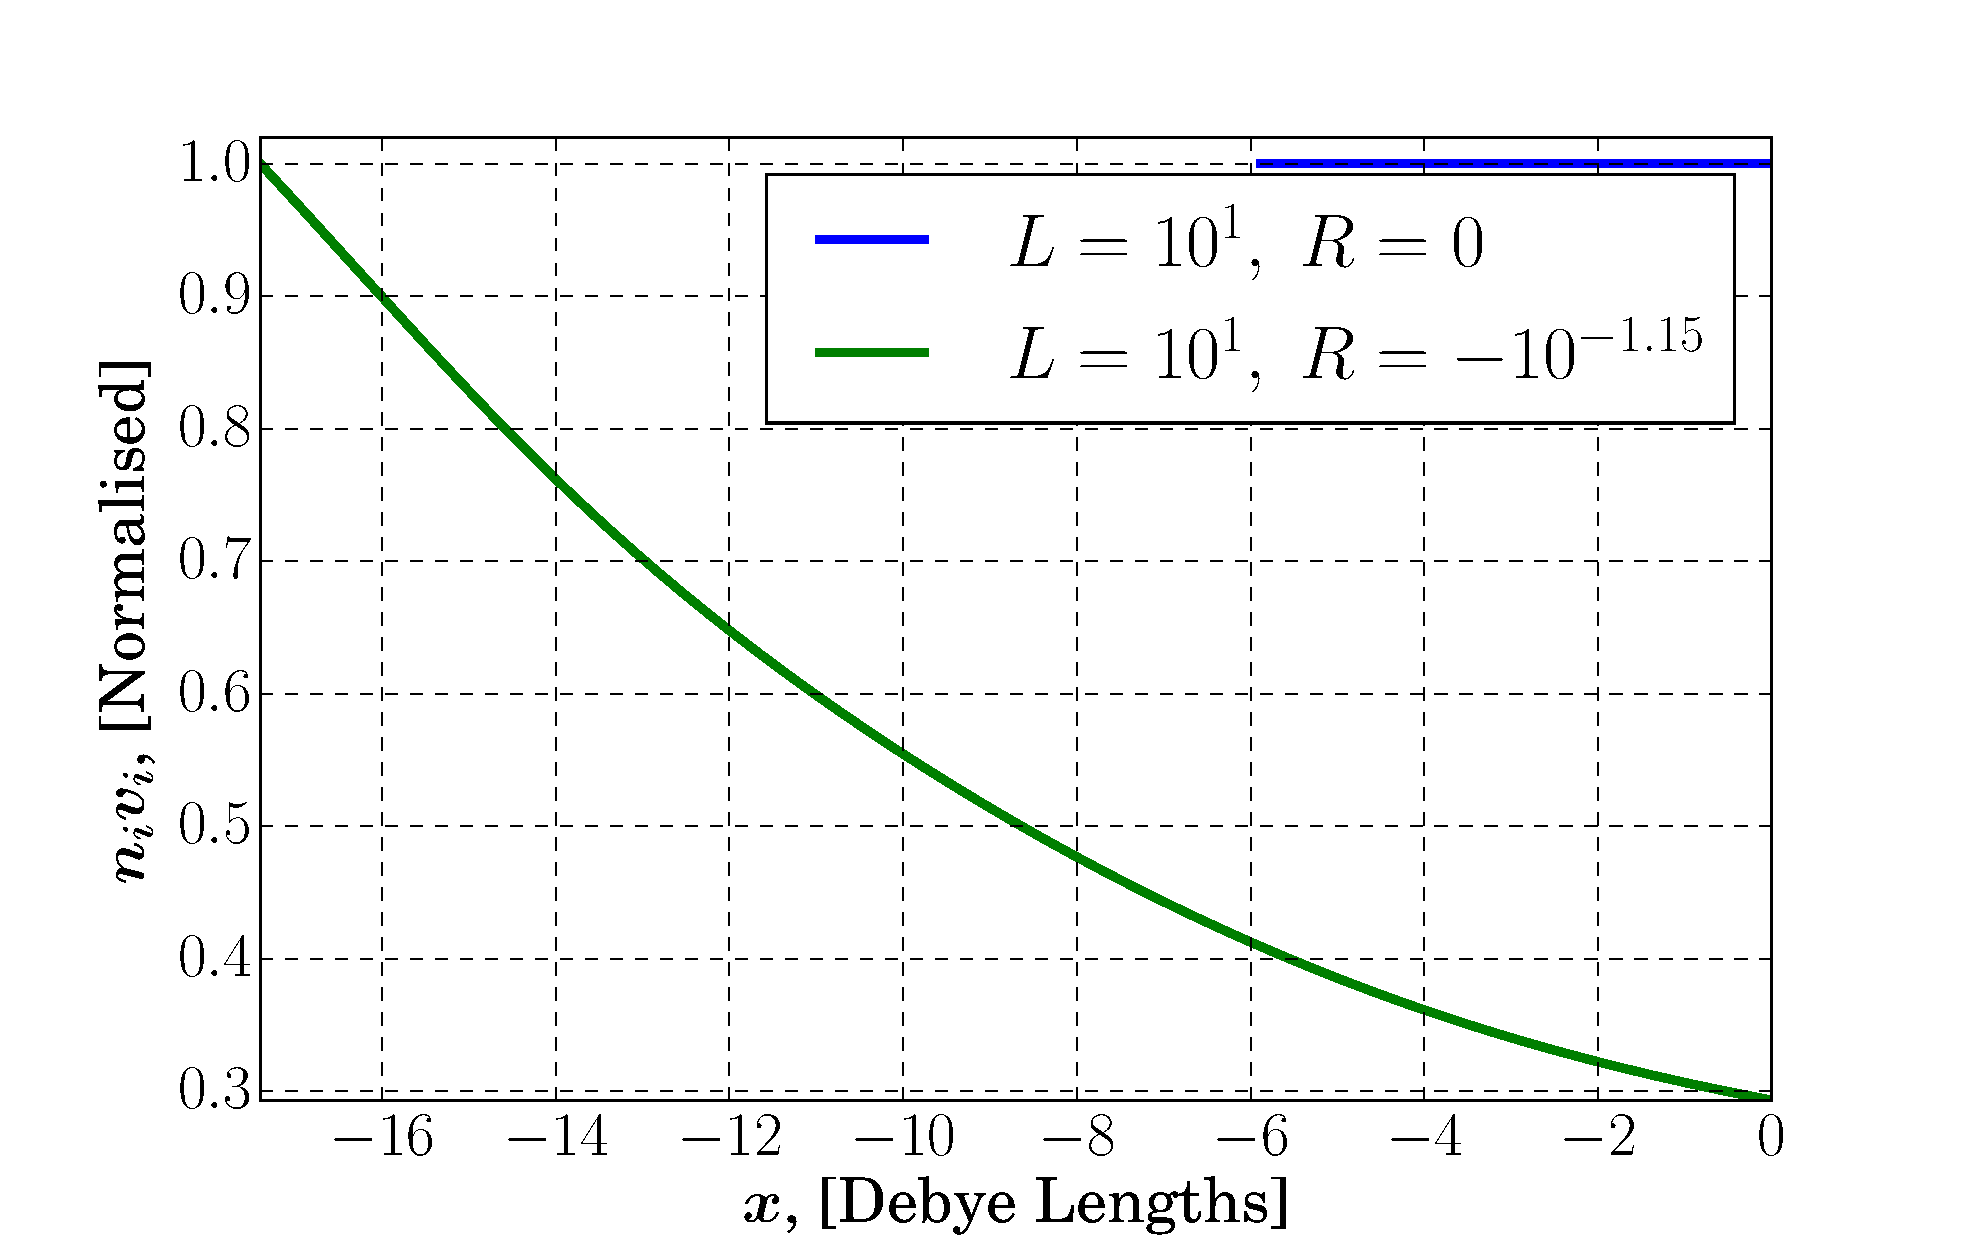
\includegraphics[width=0.3\linewidth]{6_1l.eps}
			\caption{$ L = 10 $.}
		\end{subfigure}
		\caption{$ R = 0 \textrm{ vs. } R = -L \times 10^{0.15} $. Left to right, top to bottom: current, electrostatic potential, electric field, and ion velocity, density and continuity. All as a function of distance from the wall.}
	\end{figure}
	
	
	\begin{itemize}
		\item Description of method appropriate for a paper. Give details of anything which you have done diferently, and give references for widely known methods such as RK4
		\item Figures clearly presented. Legible labels and captions
		\item Figures numbered and referenced in the text
		\item Guidline length $\sim 2$ pages
		\item 20\%
	\end{itemize}
	
	\section{Discussion}
	\begin{itemize}
		\item Summarises main findings
		\item Discussion of the implications of your result
		\item Relates results to literature and introduction
		\item Guidline length $ \dfrac{1}{2} \to 1 $ page
		\item 20\%
	\end{itemize}
	
	\section{References}
	Use academic books and articles as references, 20\%.
	
	\section{Structure and presentation}
	\begin{itemize}
		\item Good use of English
		\item Clear, legible layout
		\item Each section is relevant to the next, and sections refer to each other where appropriate
		\item 20\%
	\end{itemize}
	\bibliography{aipsamp}
\end{document}